By taking a recurrence from ergodic trajectories using a crude Poincar\'e section
formulation, and then using convolution with a Gaussian mollifier yields bad
spatiotemporal results. Due to the discrepancy between the few steps of convergence
it takes for known orbits and the complete lack of convergence for the few new orbits
tried it seems to indicate that either the initial Newton residual for convergence has
to be smaller than what I am starting with. $10^{-3}$ seems to be the maximum
for the initial residual value.

Began parsing through the literature on (variational) {newton descent},
specifically \refrefs{CvitLanCrete02,lanVar1} and for invariant tori
\refref{LCC06}.
\beq
\frac{\partial x}{\partial \tau}(s + \omega, \tau) + \frac{\partial x}{\partial s}(s + \omega, \tau)\frac{\partial \omega}{\partial \tau}(\tau) - J(x(s,\tau))\frac{\partial x}{\partial \tau}(s,\tau) =
f(x (s,\tau))-x(s+\omega,\tau),
\ee{MNGNewtonDescent}
Still trying to find a systematic way of producing initial conditions for
the use of variational {newton descent}. The main equation governing the
fictitious time evolution is again \refeq{e-MNGVND} or the non-square
matrix variant, \refeq{e-MNGVNDpseudo}. The only differing components
from that of the R\"ossler system, or spatial \KS\ is the definition of
the velocity field $v$ and therefore the definition of the stability
matrices $A$.

Began parsing through the literature on (variational) {newton descent},
specifically \refrefs{CvitLanCrete02,lanVar1} and for invariant tori
\refref{LCC06}.
\beq
\frac{\partial x}{\partial \tau}(s + \omega, \tau) + \frac{\partial x}{\partial s}(s + \omega, \tau)\frac{\partial \omega}{\partial \tau}(\tau) - J(x(s,\tau))\frac{\partial x}{\partial \tau}(s,\tau) =
f(x (s,\tau))-x(s+\omega,\tau),
\ee{MNGNewtonDescent}
Still trying to find a systematic way of producing initial conditions for
the use of variational {newton descent}. The main equation governing the
fictitious time evolution is again \refeq{e-MNGVND} or the non-square
matrix variant, \refeq{e-MNGVNDpseudo}. The only differing components
from that of the R\"ossler system, or spatial \KS\ is the definition of
the velocity field $v$ and therefore the definition of the stability
matrices $A$.

There is a storm in the distance however, as this general procedure is ruined for the spatial problem.
As we know from the chronotopic literature \refrefs{LePoTo96, LePoTo97, PoToLe98, GiLePo95},
that iteration in space typically does not converge to the same attractor as iteration in time,
and generally corresponds to a strange repeller. Therefore I cannot hope to form an initial
guess loop from using a Poincar\'e section in the spatial direction, as typically all of my
Fourier coefficients go off to infinity before a recurrence is found.

My idea to remedy this is to actually use \emph{time} integration to form a
initial guess loop for applying {newton descent} in \emph{space}. If I integrate a spatially
periodic initial condition in time, by virtue of the spatial periodicity there is a
close recurrence in the spatial direction (close and not exact only due to discretization I believe).
If I've thought about this the right way. It's the smartest way I can think of to
generate an initial condition for the spatial {newton descent} \refeq{e-FksX} given
that my spatial integration code is ill-behaved. If my \emph{spatial} code was
working and there is no lapse in my rationale then it might actually have been
a way to produce smooth initial guess loops for the \emph{time} direction {newton descent} code.

For any changes that I make that translate generically to
any system I try to test them with R\"ossler first before applying them
to antisymmetric subspace $\bbU^+$ of \KS. The other changes that are
unique to antisymmetric \KS\ must of course be tested in that realm. The
changes are looking promising, as I can find longer periodic orbits in
the R\"ossler system now, however the period seems to be slightly off
(Integrating the solution after application of {newton descent} yields a
solution that is periodic but overlaps). This is my number one suspect
for why the {newton descent} code continues to stall at the moment; however,
for the R\"ossler system although it is much slower for longer periodic
orbits, it still converges very quickly once $F^2 < 1$.

I realized that I should not have to worry about implementing a slicing condition
in the spatial version of variational {newton descent}; All that was required in the
time case was to reduce the symmetry associated with the marginal direction parallel to
velocity, i.e. a Poincar\'e section. I didn't worry about the spatial translational invariance
and it was able to converge to a solution just fine in the time case.
There also might be a smarter way of choosing a constraint that enables better
convergence, as opposed to the ``first coordinate" hyperplane (i.e. the first
Fourier mode in most systems). I'm currently playing around with using a
hyperplane condition on the ``more dynamical" variables \MNGedit{which is a
hasty and crude name not to be taken seriously}. What I mean by this is that in
\refeq{e-FksX} the spatial derivatives of the Fourier coefficients of
$u^{(3)}$, which represents the third derivative, are much more complex than
the other derivatives, so perhaps using a hyperplane condition on one of these
coordinates would be better; this hasn't seemed to be the case yet.

I thought that I would have to somehow permute the elements \refeq{e-FvndBAD} of the "Loop Vector" (vector that
encodes the parameterization of initial condition for periodic orbit search). The reasoning behind this
was in order to use differentiate with respect to a parameterization variable $s$, I would need
the elements to be in sequential order with respect in parameterization variable $s$, in order to
multiply by vector $i \vec{m}$, where $m$ is the conjugate variable (in a Fourier transform sense)
to $s$. This is \textbf{\emph{not}}
the case, as I can merely exploit the Kronecker outer product to produce a diagonal matrix such that
along the diagonal there are $M$ duplicates of each element of $\vec{m}$

We are essentially diagonalizing a sparse matrix for $\mathcal{O}(M\,(n log(n)))$ flops
from taking $M$ Fourier transforms of length $n =$~power~of~$2$.
This is all well and good, but I think that there might be complications from the stability matrices;
I need to go through the calculation, but the naive way to write the
stability matrices in their new representation is:
 $\tilde{\mathbf{A}} = \mathbf{F} \mathbf{A} \mathbf{F^{*}}$, where $F$
is a unitary matrix representing the discrete Fourier transform.

Next is the representation of the fictitious time evolution as a system of linear equations, similar to
\refeq{e-MNGVNDpseudo}, which is restated here for comparison to the new system of equations.

The old linear system is given by,
\beq
\begin{bmatrix} M & -v \end{bmatrix}  \left[ \begin{array}{c} \delta \tilde{x} \\ \delta \lambda \end{array} \right] =
    \delta \tau \left[ \begin{array}{c} \lambda v - \tilde{v} \end{array} \right],
\eeq
where $M = D - \lambda Diag(A_n)$ with $D$ being the finite difference matrix, and $A_n$ a block diagonal matrix containing stability matrices.

Now, the equations the same form, with new variables described by over-bars
\beq \label{e-MNGVNDpseudoFMAT}
\begin{bmatrix} \bar{M} & -\bar{v} \end{bmatrix}  \left[ \begin{array}{c} \delta \tilde{\bar{x}} \\ \delta \bar{\lambda} \end{array} \right] =
    \delta \tau \left[ \begin{array}{c} \lambda \hat{\bar{v}} - \tilde{\bar{v}} \end{array} \right],
\eeq
where $\bar{M} = \mathbf{F} Diag (i \vec{m}) \mathbf{F}^* \otimes \mathbf{I}_d - \lambda Diag(A_n)$
%$\bar{M} = Diag (i \vec{m}) \otimes \mathbf{I}_d - \lambda \mathbf{F} Diag(A_n) \mathbf{F}^*$,
and $\bar{v} = \mathcal{F}(v)$, $\tilde{\bar{v}} = (Diag(i \vec{m})* \tilde{\bar{x}}$.
\MNG{}{I changed this such that the only difference
between my current code and this formulation
 is the calculation of approximate tangent space via Fourier methods.}


After talking to Ashley, who told me to start the multishooting
effort with only a few number of points rather than the large
discretization used as if it was a {newton descent}, I looked back
into the variational multishooting technique that he described back
in Santa Barbara. I took four point on the original orbit, while
my code is minimizing the cost functional \refeq{e-MultishootCost}
I am yet again getting the ``equilibrium descent" for an antisymmetric initial
condition $\in \bbU^+$ that converges with my variational {newton descent} code.
This resulting equilibrium "solution" is a typical result when
something is ill-defined. I would speculate that the manner in which
I am handling the adjoint equations is the culprit, as I tried to
modify the ETDRK4 of \refref{ks05com} to be the numerical integration
routine to integrate the equations.

Fixed memory issue by making it such that the
"Newton descent matrix" i.e. the matrix in is not evaluated
before each least squares evaluation; rather, we keep this matrix
constant as an approximation and then when the cost functional
can no longer decrease, i.e. we have left the local neighborhood of
the stability matrices that define the matrix, we redefine the matrix
and then restart the search; this is similar to what is implemented
in other variational Newton descent code; forgot this fact when I
rewrote the spatial Newton descent code to use LSQR to solve the
least squares problem as opposed to using matrix inversion.
Application of the spatial Newton descent code to ergodic trajecto-
ries that have been deformed to be periodic in time were resulting in

Debugging and changing spatial {newton descent} code.
I think I've pinned down the main problem
to be an error in trying to use Fourier transforms
rather than explicit sums in my definition
for the stability matrix elements, or initial
condition generation. I'm currently using the
shortest periodic orbit in time as an initial
guess; Therefore, I would expect the value
of the cost functional to be small relative to
something that isn't already doubly-periodic
in time and space. While the value of the cost
functional is relatively small, it still may
be too large for an initial guess.
That being said I can at least list what I
 believe to be the most likely cause of errors.

The reason for this is such: Spectral differentiation with respect to a parameterization variable,
$s$, can be rewritten as multiplication by a diagonal matrix with elements $is$, but this requires
the vector that is representing the entire loop to be ordered in a very specific way. If the loop
was ordered in this specific way it would reduce to multiplication of a large diagonal matrix which would
be repeating the (small) diagonal matrices with elements $is$. If one wants to do it this way I believe
the easiest way, in order to avoid reordering the stability matrix elements, would be to formulate it
this way mathematically: The matrix $D_{\mathcal{F}}$, which produces the approximate tangent space
after multiplication with the "loop vector" $\mathbf{x}$, could be represented in such a way,

\beq \nonumber
D_{\mathcal{F}} = \mathbf{P}^{-1}\mathbf{F}^{-1}\mathbf{Diag}(is)\mathbf{F}\mathbf{P} \quad
    \mbox{where,}
\label{e-FvndBAD}
\eeq

$\mathbf{F}$ = Block diagonal matrix composed of Fourier transform matrices (i.e. to Fourier transform each
of the Fourier coefficient series with respect to parameterization variable), $\mathbf{P}$ = Permutation matrix
to reorder in specific way to enable easy Fourier transforms.

Another main challenge is how to implement a slice condition to deal with translational
invariance. Typically this is dealt with when the spatial Fourier series is being used, and
therefore it is easier to represent a hypersurface that eliminates this marginal direction; in
the spatial {newton descent} code (this is what I call using \refeq{e-FksX} with variational
{newton descent}) I am trying to eliminate the translational freedom but it's not as straightforward as
the {\fFslice}; as the {\fFslice} in this case would eliminate time translations.
I've been looking towards some of the papers about invariant tori and their "phase conditions" as a
possible means of escape.

I realized that I should not have to worry about implementing a slicing condition
in the spatial version of variational {newton descent}; All that was required in the
time case was to reduce the symmetry associated with the marginal direction parallel to
velocity, i.e. a Poincar\'e section. I didn't worry about the spatial translational invariance
and it was able to converge to a solution just fine in the time case.

I thought that I would have to somehow permute the elements \refeq{e-FvndBAD} of the "Loop Vector" (vector that
encodes the parameterization of initial condition for periodic orbit search). The reasoning behind this
was in order to use differentiate with respect to a parameterization variable $s$, I would need
the elements to be in sequential order with respect in parameterization variable $s$, in order to
multiply by vector $i \vec{m}$, where $m$ is the conjugate variable (in a Fourier transform sense)
to $s$. This is \textbf{\emph{not}}
the case, as I can merely exploit the Kronecker outer product to produce a diagonal matrix such that
along the diagonal there are $M$ duplicates of each element of $\vec{m}$

We are essentially diagonalizing a sparse matrix for $\mathcal{O}(M\,(n log(n)))$ flops
from taking $M$ Fourier transforms of length $n =$~power~of~$2$.
This is all well and good, but I think that there might be complications from the stability matrices;
I need to go through the calculation, but the naive way to write the
stability matrices in their new representation is:
 $\tilde{\mathbf{A}} = \mathbf{F} \mathbf{A} \mathbf{F^{*}}$, where $F$
is a unitary matrix representing the discrete Fourier transform.

Next is the representation of the fictitious time evolution as a system of linear equations, similar to
\refeq{e-MNGVNDpseudo}, which is restated here for comparison to the new system of equations.

The old linear system is given by,
\beq
\begin{bmatrix} M & -v \end{bmatrix}  \left[ \begin{array}{c} \delta \tilde{x} \\ \delta \lambda \end{array} \right] =
    \delta \tau \left[ \begin{array}{c} \lambda v - \tilde{v} \end{array} \right],
\eeq
where $M = D - \lambda Diag(A_n)$ with $D$ being the finite difference matrix, and $A_n$ a block diagonal matrix containing stability matrices.

Now, the equations the same form, with new variables described by over-bars
\beq \label{e-MNGVNDpseudoFMAT}
\begin{bmatrix} \bar{M} & -\bar{v} \end{bmatrix}  \left[ \begin{array}{c} \delta \tilde{\bar{x}} \\ \delta \bar{\lambda} \end{array} \right] =
    \delta \tau \left[ \begin{array}{c} \lambda \hat{\bar{v}} - \tilde{\bar{v}} \end{array} \right],
\eeq
where $\bar{M} = \mathbf{F} Diag (i \vec{m}) \mathbf{F}^* \otimes \mathbf{I}_d - \lambda Diag(A_n)$
%$\bar{M} = Diag (i \vec{m}) \otimes \mathbf{I}_d - \lambda \mathbf{F} Diag(A_n) \mathbf{F}^*$,
and $\bar{v} = \mathcal{F}(v)$, $\tilde{\bar{v}} = (Diag(i \vec{m})* \tilde{\bar{x}}$.
\MNG{}{I changed this such that the only difference
between my current code and this formulation
 is the calculation of approximate tangent space via Fourier methods.}

The best results, (i.e. better than square matrix problem, but still not
good enough) was with SciPy's LSQR algorithm, which, in the paper that
it is based on \refref{PaSaLSQR}, describes it as a ``conjugate-gradient-like" algorithm,
with better stability. I haven't gotten into the nitty gritty as of yet.

While waiting for Arnoldi iteration to finish so that I could begin testing the
spatial variational {newton descent} without fear of memory problems I was trying to
think about the best way to use \refeq{e-FksSpattemp}, which I will restate
here:
\beq
\left[ i \omega_\ell - ( q_k^2 - q_k^4 ) \right]\utensor_{k,\ell}
+ i \frac{q_k}{2} \!\sum_{k'=0}^{N-1} \sum^{M-1}_{m'=0}\!\!
\utensor_{k',m'} \utensor_{k-k',m-m'}
    =
0
\,.
\eeq
First, $\utensor_{k,\ell}$ represents matrix elements, so it makes sense
to rewrite the equation as a matrix equation. Define matrices
$\mathbf{Q}_1 \equiv Diag(-q_k^2 +q_k^4)$,
$\mathbf{W} \equiv Diag(i \omega_\ell)$,
$\mathbf{Q}_2 \equiv Diag(\frac{i q_k}{2})$, and let
the two dimensional FFT be represented by matrix multiplication
$\mathbf{U} = \mathbf{F}_M \mathbf{u} \mathbf{F}_N$,
where the matrix elements $U_{k,\ell} = \utensor_{k,\ell}$.

With these definitions the equation can be rewritten as:
\beq
\mathbf{Q_1} \mathbf{U} \mathbf{W} + \mathbf{Q_2}\mathbf{F_M}(\mathbf{u} \otimes \mathbf{u})\mathbf{F_N} = 0
\label{e-FksSpattempMat}
\eeq
where the nonlinear term is calculated in configuration space as to avoid the two dimensional convolution.

Because $\mathbf{Q_1}$ and $\mathbf{W}$ are diagonal, their inverses are easily found, and the equation \refeq{e-FksSpattempMat} can be rewritten

\beq
\mathbf{Q_1}^{-1} \mathbf{Q_2}\mathbf{F_M}(\mathbf{u} \otimes \mathbf{u})\mathbf{F_N}\mathbf{W}^{-1} + \mathbf{U} = 0
\eeq
Now we can redefine $\mathbf{U} \rightarrow -\mathbf{U}$, and remember to convert
back after finding the fixed point.

Define
\beq
f_{k,\ell}(\utensor_{k,\ell}) \equiv \mathbf{Q_1}^{-1} \mathbf{Q_2}\mathbf{F_M}( \mathbf{u} \otimes \mathbf{u}) \mathbf{F_N} \mathbf{W}^{-1}
\eeq
and therefore we have an equation of the form:
$f_{k,\ell}(\utensor_{k,\ell})-\utensor_{k,\ell} = 0$,
where the \jacobianM\ is given by the fourth rank tensor that arises from taking partial derivatives with
respect to $\utensor_{k,\ell}$
More to be derived in the future, hoping to make headway into finding tori; I can't tell if this equation
is going to be useful or if I should really be working towards deriving and learning variational {newton descent}
equations for finding tori similar to Lan, Chandre and Cvitanovi{\'c}\rf{LCC06}.

Application of the spatial {newton descent} code to ergodic trajectories that have been deformed to
be periodic in time were resulting in the "falling into equilibrium" problem, this was due to a bug
where the wrong temporal system sizes were being used.

Application of spatial {newton descent} on \ppo{10.2} results in a reduced cost
functional but seems rather obstinate in regards to convergence. Luckily, the
approximate loop seems to fluctuate around spatial extent $L=22$. I think this
is a good indication as it means the spatial {newton descent} is capturing the
spatial geometry of \ppo{10.2}. That is to say, even while reducing the cost
functional the solution doesn't want to betray itself, as it originates from
the spatial system size $L=22$.

I tried whether it be the error tolerances, step sizes (variable or constant), initial condition
discretizations, least squares solvers, pseudoinverse or regular inverse methods, hypersurface constraints,
matrix preconditioners, etc, did not help the converge properties.
By examining the corrections being applied to deform the loop, specifically the maximum correction applied
in each step it seems most of the steps are modifying the "period" i.e. the spatial extent of the initial
condition the most. There might be some way to discourage this with an additional condition on the
rescaling factor $\lambda$ that matches the magnitudes of the approximate tangent space to the
actual tangent space.
The majority of modifications being put into changing this rescaling factor seem to be the cause of
the critical slow down of the algorithms, which might be indication of the presence of a continuous
symmetry that needs to be dealt with that isn't currently being dealt with.

Still haven't been able to get this to work, after some thought over the weekend
I have been trying to implement a major change to the code. The general idea is this,
the first three equations of \refeq{e-FksX} will by definition match the approximate
loop tangents as they are generated via spectral differentiation, which is now
how I am computing the approximate loop tangents. I have been trying to work out how
this can be exploited as to greatly reduce the dimensionality of the system. I.e. instead
of keeping track of the real and imaginary components of the Fourier coefficients
of $u, u_x, u_{xx}, u_{xxx}$, I should be able to only keep track of $u$, and then match
the last equation of \refeq{e-FksX} to the fourth derivative of u computed by spectral
differentiation. The main problem with this formulation is that I haven't been able to
rewrite figure out the best way to rewrite the stability matrix elements, other than they
should only depend on the real and imaginary components of the temporal Fourier modes of $u$.

The key idea is that because the initial conditions for the spatial system,
$u, u_{x}, u_{x x}, u_{x x x}$ were all being generated
through spectral differentiation, it made matching the tangent spaces redundant in
three variables, as the approximate tangent spaces were being generated with spectral
differentiation as well. Therefore, the idea is to turn only the last equation in
\refeq{e-FksX} into a ``direct-matrix" \rf{Chu09} equation similar to the spatiotemporal mapping,
and match it to the velocity field's fourth derivative.
By proceeding in this manner, the equation for the fourth derivative, (which I will
refer to from here on as \emph{the} tangent space) takes the following ``direct-matrix"\rf{Chu09} form.
Note, that I am attempting to devise an equation that is only dependent on the Fourier coefficient of the
velocity field and not any of the spatial derivatives. This is acceptable because the spatial derivatives
are derived from the original velocity field anyway. What appears now in the equations are linear operators
that produce the derivatives accordingly. Therefore, $\utensor$ will refer to $\utensor^{0}$ in accordance with
notation previously used. Finally, the velocity equation (fourth spatial derivative) now appears as follows,

The key idea is that because the initial conditions for the spatial system,
$u, u_{x}, u_{x x}, u_{x x x}$ were all being generated
through spectral differentiation, it made matching the tangent spaces redundant in
three variables, as the approximate tangent spaces were being generated with spectral
differentiation as well. Therefore, the idea is to turn only the last equation in
\refeq{e-FksX} into a ``direct-matrix" \rf{Chu09} equation similar to the spatiotemporal mapping,
and match it to the velocity field's fourth derivative.
By proceeding in this manner, the equation for the fourth derivative, (which I will
refer to from here on as \emph{the} tangent space) takes the following ``direct-matrix"\rf{Chu09} form.
Note, that I am attempting to devise an equation that is only dependent on the Fourier coefficient of the
velocity field and not any of the spatial derivatives. This is acceptable because the spatial derivatives
are derived from the original velocity field anyway. What appears now in the equations are linear operators
that produce the derivatives accordingly. Therefore, $\utensor$ will refer to $\utensor^{0}$ in accordance with
notation previously used. Finally, the velocity equation (fourth spatial derivative) now appears as follows,

\beq \label{e-FksXdirectmatrix}
v = -W \dot \utensor - Q_2 \dot \utensor - F \dot ((F^{-1}\dot \utensor) \star ((F^{-1}\dot Q1 \utensor)),
\eeq

Using the direct-matrix differentiation rules noted above \refeq{e-DMdiffrules}, the stability matrix takes on the following form,

\beq \label{e-FksXdirectStbMat}
A = - W - Q_2 - F \dot (diag(F^{-1}\dot Q1 \dot \utensor)\dot F^{-1} + diag(F^{-1} \dot \utensor) \dot F^{-1} \dot Q1)
\eeq

For a quick description of the operators, $W$ is the operator that produces the time derivative of a given field
$\utensor$, $Q_2$ produces the second spatial derivative, $F$ performs a forward FFT of a time-series, $Q_1$ produces
the first spatial derivative. In this notation, the approximate tangent space would be the fourth spatial derivative
as produced by spectral differentiation, i.e. $\tilde{v} = Q_4 \dot \utensor$. Everything else from the variational
{newton descent} is left untouched.

I'm hoping that this will enable convergence of the spatial system of equations to find periodic orbits in space, the
main motivation for performing these changes were firstly, the code wasn't working probably due to some inaccuracies or errors,
secondly, by keeping
everything defined in terms of only the original velocity field $u(x, t)$ I dramatically reduce the memory
requirements and degrees of freedom of the system.

Spent the day debugging the spatial {newton descent} code, found a negative sign error in the expression for
matrices governing Fourier transforms, converted from taking real(cosine and sine) fft's in one variable (time) to complex fft's
as I was having some trouble reproducing the time derivative term otherwise. Took a while to figure out what was wrong until
I looked at matrix-product results piece by piece and compared to expected results in MATLAB. Rewrote how matrices (derivative
operators) are formulated in terms of the Fourier transform operators. Also found a peculiarity when it came to the accuracy
of matrix multiplcation depending on the order in which the matrices were multiplied...haven't figured that one out yet but nonetheless
I corrected it.

I believe I got it working finally, however, the results so far aren't as
interesting as I had dreamed. I finished this at the end of the day so I didn't
get to test it too much, but so far there are two resulting possibilities.
First, with a time periodic initial condition, i.e. one of the periodic orbits
in time of \KS, when allowing for spatial domain changes and changes to the
temporal Fourier coefficients, the solution (only tested one so far) converged
to one of the temporal equilibria of the \KS\ system. This I believe is an
indication that my code is indeed working, even though this was usually a sign
of numerical issues when searching for periodic orbits in time using the
variational methods, (i.e. the only way to reduce the cost functional
$\mathcal{F}^2 = \lambda v - \tilde{v}$ is to send $v$ and $\tilde{v}$ to $0$.
The reason I believe this is still valid is because the spatial derivatives of
the equilibrium state found are nonzero; i.e. one of the "spatial periodic
orbits" I have found is indeed the temporal equilibrium of the system.

When using a coarse discretization of 16-by-16 space-by-time points
the spatial domain size that the solution settled to was $L=19.9324743429$, with the
value of cost functional being within machine precision of $0$.
When the spatial discretization was doubled, i.e. a 32-by-16 space-by-time
grid, the resulting domain size was $23.7360639824$.
Likewise, when using a 16-by-32 space-by-time discretization, the resulting domain size was $L=19.9398768032$, which indicates that the
domain size of the converged solution is highly dependent on the (spatial)discretization being using.

The second possibility is a convergence to a zero domain size solution, which in my variational method for time usually indicated an equilibrium of
the system. I.e. the two possibilities were either an equilibrium in time (but still a periodic orbit in space), or a spatial equilibrium.

After more investigation it turns out that the spatial variational code is indeed not working yet. Tried to put
resulting orbits into time integrator in order to reproduce the result and got an unmatching solution.
\reffig{fig:MNGvndspace2} is my
newest "results". It uses a \RPO{16.31} of the \KSe\ as the initial condition. I think I was deceived by how nice it looks
I suppose...couldn't find any errors today that could enable reproduction via time integration.

As an additional test I put the solutions into Burak's symmetry reduced time integrator to verify whether
the "solution" in \reffig{fig:MNGvndspace2} was a \rpo\ but alas there was no luck; there is some other error
that I haven't been able to identify as of yet.
Found another negative sign error, updating \reffig{fig:MNGvndspace1}.

Applied changes based on implementation from spatial variational method to my torus finding code but it seems
I jumped the gun as I cannot reproduce any orbits found by spatial {newton descent} via time integration.

\begin{figure}[ht]
\begin{minipage}[height=.32\textheight]{.45\textwidth}
\centering \small{\texttt{(a)}}
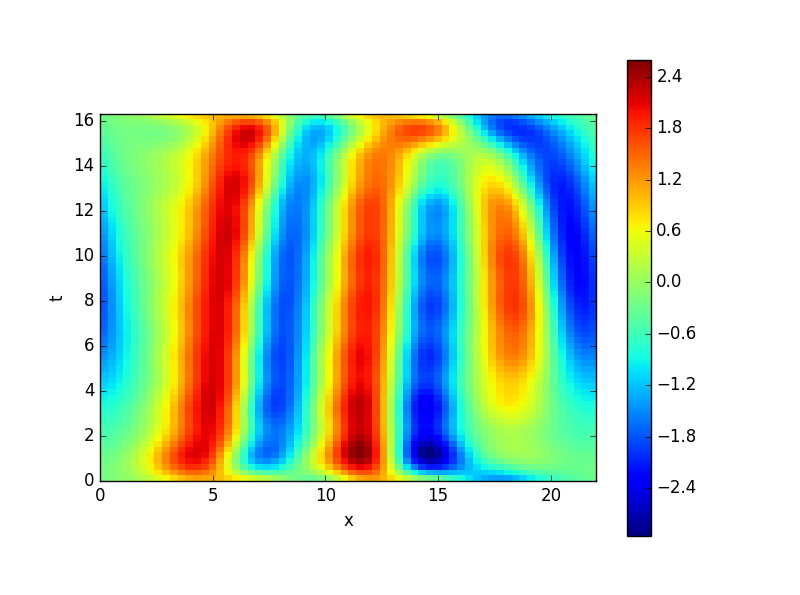
\includegraphics[width=\textwidth,height=.32\textheight]{MNGvndspaceinit2}
\end{minipage}
\begin{minipage}[height=.32\textheight]{.45\textwidth}
\centering \small{\texttt{(b)}}
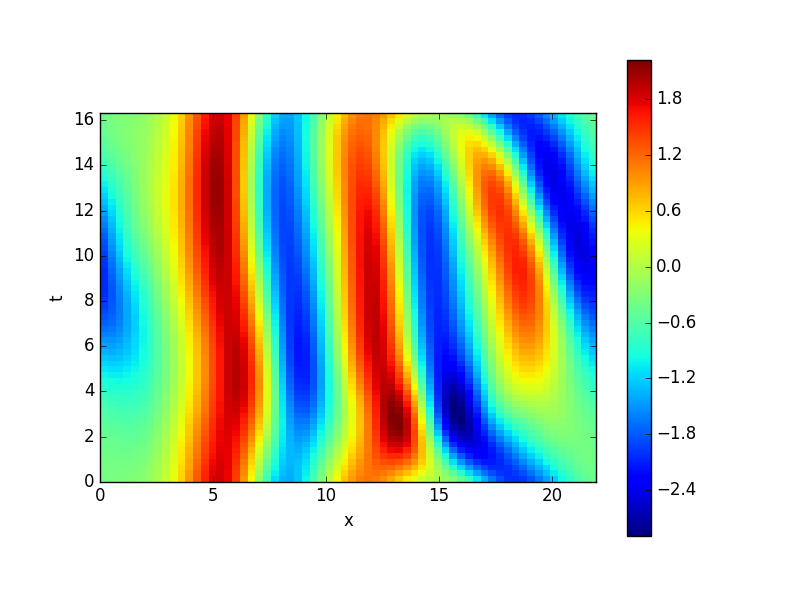
\includegraphics[width=\textwidth,height=.32\textheight]{MNGvndspacefinal2}
\end{minipage}
\caption{ \label{fig:MNGvndspace2}
(a) Initial condition of the 16-by-16 space-by-time discretization of \RPO{16.31} ($L=22$) for spatial
variational {newton descent} of the \KSe\ (b)Resulting "spatial periodic orbit" (temporal equilibrium), with
final spatial extent of $L = 21.9394614064$
}
\end{figure}
\begin{figure}[ht]
\begin{minipage}[height=.32\textheight]{.45\textwidth}
\centering \small{\texttt{(a)}}
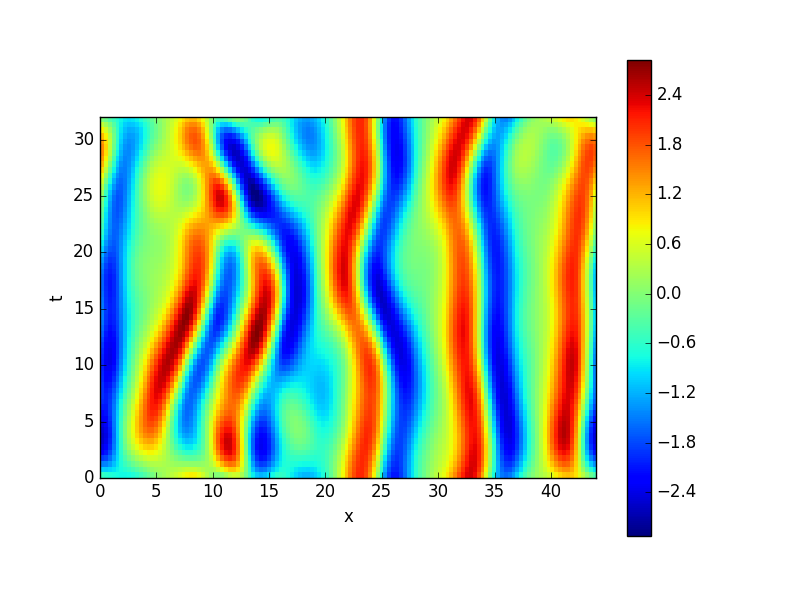
\includegraphics[width=\textwidth,height=.32\textheight]{MNGvndspaceinit3}
\end{minipage}
\begin{minipage}[height=.32\textheight]{.45\textwidth}
\centering \small{\texttt{(b)}}
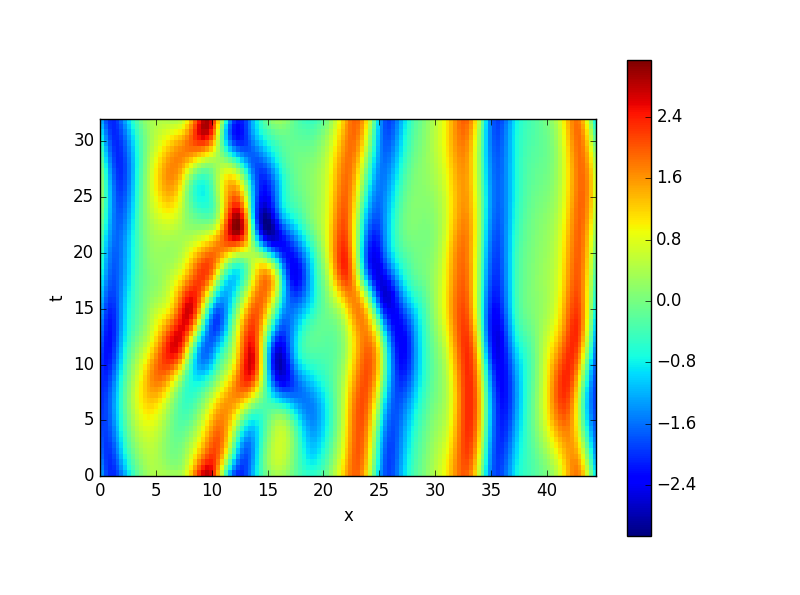
\includegraphics[width=\textwidth,height=.32\textheight]{MNGvndspacefinal3}
\end{minipage}
\caption{ \label{fig:MNGvndspace3}
(a) Initial condition of the 32-by-16 space-by-time discretization of a piece
of an ergodic trajectory that has been deformed to be periodic in time. $L=44$.
(b) Resulting spatiotemporal \po, with
final spatial extent of $L = 44.3937151766$.
}
\end{figure}


updated \reffig{fig:MNGvndspace2}, \reffig{fig:MNGvndspace1}, and uploaded \reffig{fig:MNGvndspace3} to display
current results.

After trying numerous small modifications to the variational method's system
of equations from \refref{LanThesis} including implementing factors involving
the coordinate involved in defining the in-slice time and other quantities
involving the slice tangents I didn't get any improvements over what I already
had. I still think the problem has to do with the slice time so I went over
the derivation of the equations and I believe I found a correction that can be
made.

The derivation of the system of equations used to find the fictitious time
corrections to the initial guess loop involves substitution of the
partial derivative of the rescaling factor with respect to fictitious time.
The way that this is done is via the definition

\beq
\lambda_n = \frac{\Delta \tn }{\Delta s_n} \, ,
\eeq
where, $s$ is the parameterization variable, here defined with a subscript $n$
to indicate that the parameterization need not be uniform around the initial guess
loop (although this is what I work worth as it makes things much easier to program).
$t$ in this instance stands for the real dynamical time of the orbit.

If we substitute the definition for the in-slice time, this equation takes the form

\beq
\lambda_n = \frac{\Delta \hat(t)_n (x_1)_n }{\Delta s_n}
\eeq

Going through the almost identical derivation for the system of equations there
is one place where I believe they differ. Normally, there is the substitution

\beq
\delta \tn = \frac{\partial \lambda_n}{\partial \tau} \Delta s_n \delta \tau
\eeq

Normally this is easily generalized in order to produce a uniform rescaling of the period
around the orbit,
but if the coordinate $x_1$ is involved I believe that this should take the form

\beq \label{e-inslicevarmeth}
\delta \tn = (\frac{\partial \lambda_n}{\partial \tau}(x_1)_n + \frac{\partial (x_1)_n}{\partial \tau} \lambda_n)\Delta s_n \delta \tau
\eeq

As the in-slice time rescaling is coordinate dependent, this formula seems to beg for a description
of the general equation that has a coordinate dependent rescaling. This is kind of what I have been stuck on
as this is quite different from what I am used to.

For a orbit that is described by $M$ points in time we would need ${\lambda_i}$ where $i = 0, ... , M-1$.
I'm currently working on implementing this into my current code but it's gotten the best of me so far.

The way I am attempting to solve the problem I am having with in-slice time is as such,
for $M$ discretized points representing an in-slice time description of a {\rpo} I am introducing
$M$ different time rescaling quantities $\lambda_m$. In this way the original variational
method equation changes from
\beq
\begin{bmatrix} D - \lambda diag(A_0, ... , A_{M-1}), & -v \end{bmatrix}
       \left[ \begin{array}{c} \delta \tilde{x} \\ \delta \lambda \end{array} \right] =
    \delta \tau \left[ \begin{array}{c} \lambda v - \tilde{v} \end{array} \right],
\eeq
to
\bea
&&\begin{bmatrix} D - diag(\lambda_0 * A_0, ... , \lambda_{M-1} * A_{M-1}), & -diag(v_0, ..., v_{M-1}) \end{bmatrix}  \left[ \begin{array}{c} \delta \tilde{x} \\ \delta \lambda_{m}
            \end{array} \right]
\continue
&&=
    \delta \tau \left[ \begin{array}{c} diag(\lambda_m) v - \tilde{v} \end{array} \right],
\eea
In this way the correction mentioned in \refeq{e-inslicevarmeth} is not being resolved but I want to try
to see if more flexibility in the rescaling of in-slice time with respect to fictitious time evolution
is sufficient before getting into an equation I derived; it's also a simpler step whose changes could be
carried over to the full in-slice time description I probably will need.

Wrote some new code for symmetry reduced spatiotemporal fixed point finding; currently
it seems a little strange to me because I only know how to quotient the spatial translation
symmetry in spatial Fourier space as opposed to spatiotemporal (double) Fourier space.

The way that this I am attempting this, are with the equations, in direct-matrix notation:

Using the definition of the reduced velocity in ti
me, \refeq{e-KSsymDMvelnew}, restated here
for reference,
\beq
\hat{v} = (X \cdot \utensor) \ast v - (\dot{Y} \cdot v) \ast (I_M \otimes T) \cdot \utensor,
\eeq
We then find the equivalent spatiotemporal system by Fourier transforming in time by means
of application of $F_t$ linear operator denoting the transform and moving everything to one
side. Here, the $\utensor$ stands for a description of the initial solution that is only Fourier in space.
\beq
W\cdot F_t \cdot \utensor -F_t\cdot((X \cdot \utensor) \ast v - (\dot{Y} \cdot v) \ast (I_M \otimes T) \cdot \utensor) = 0
\eeq
The stability matrix resulting from this symmetry reduced mapping is therefore,

where $\hat{A}$ is in reference to the equation previously defined \refeq{e-KSsymDMstbnew}.

\beq
J = W\cdot F_t - F_t\cdot \hat{A}
\eeq

The part that troubled me for a while was how to implement symmetry reduction of the spatial translation
symmetry in a spatiotemporal way as opposed to what I have now. I haven't been able to come
up with anything good yet but it just seems like a little bit of a hack job to reduce
the symmetry before taking things to the spatiotemporal stage. Because I am trying
to find fixed points after symmetry reduction I imagined that this case should be
exactly be like symmetry reduction of a \reqva\ but I haven't found a good way of treating
the equations yet.




\begin{figure}[ht]
\begin{minipage}[height=.32\textheight]{.45\textwidth}
\centering \small{\texttt{(a)}}
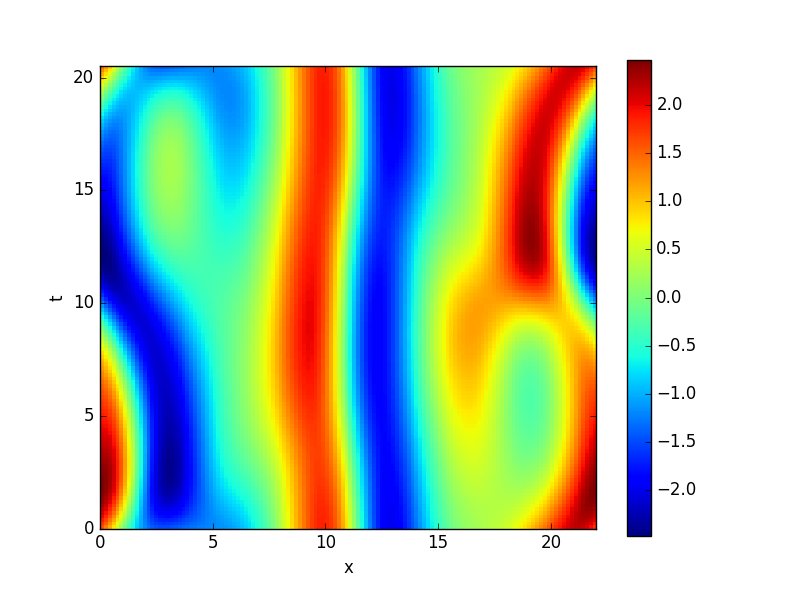
\includegraphics[width=\textwidth,height=.32\textheight]{MNGspacetimeinit1}
\end{minipage}
\begin{minipage}[height=.32\textheight]{.45\textwidth}
\centering \small{\texttt{(b)}}
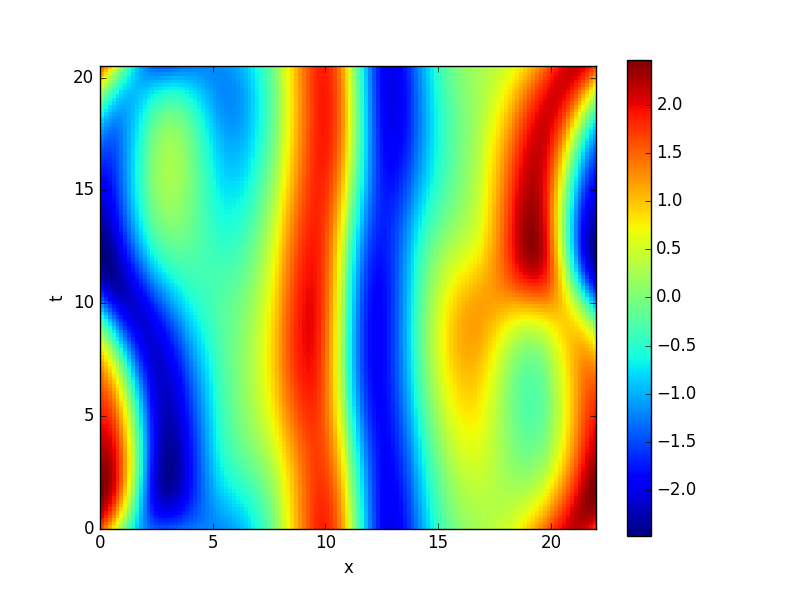
\includegraphics[width=\textwidth,height=.32\textheight]{MNGspacetimefinal1}
\end{minipage}
\caption{ \label{fig:MNGspacetime11}
(a) Initial condition of the 32-by-32 space-by-time discretization of \ppo{10.2}:
$(L_0,\period{0}) = (L_0, 2\period{p_0})= (22,20.5057459345)$.
(b) Resulting spatiotemporal fixed point
$(L_p,2\period{p}) =  (22.0000104401, 20.5057499188)$
}
\end{figure}

\begin{figure}
\begin{minipage}[height=.32\textheight]{.45\textwidth}
\centering \small{\texttt{(a)}}
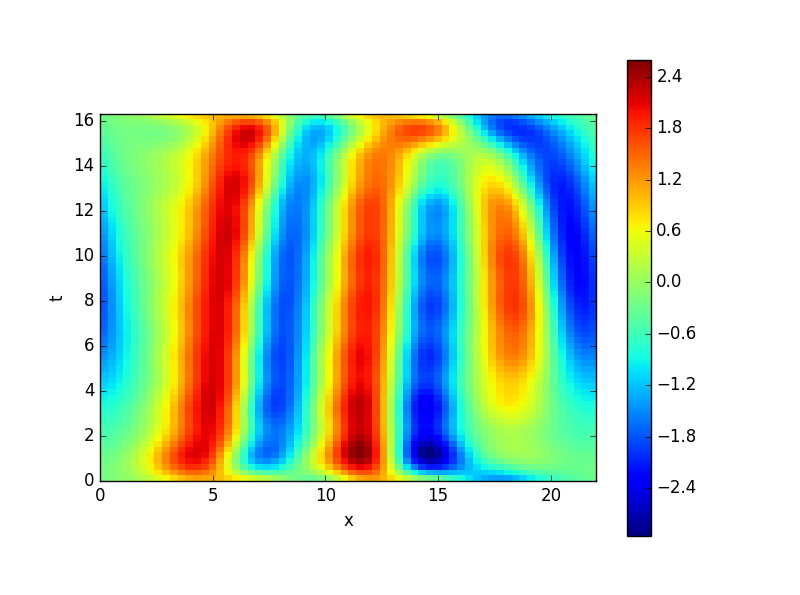
\includegraphics[width=\textwidth,height=.32\textheight]{MNGvndspaceinit2}
\end{minipage}
\\
\begin{minipage}[height=.32\textheight]{.45\textwidth}
\centering \small{\texttt{(b)}}
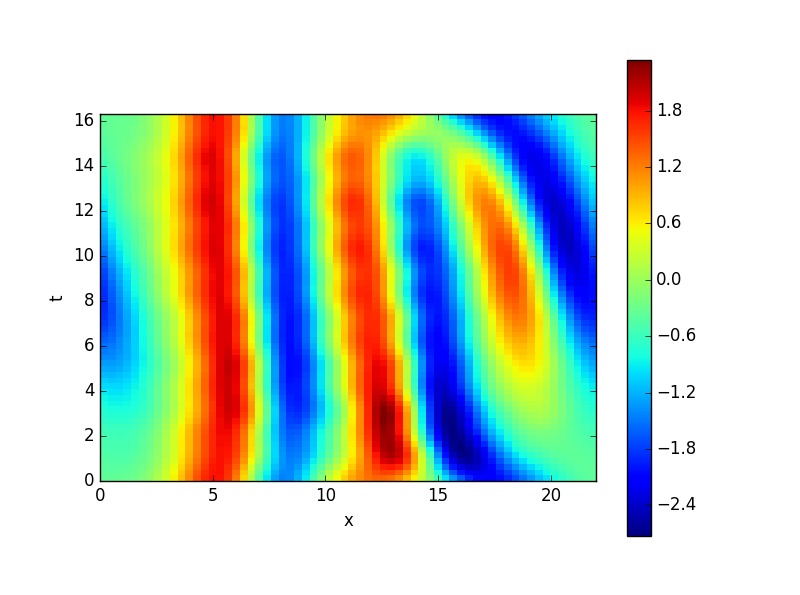
\includegraphics[width=\textwidth,height=.32\textheight]{MNGvndtimefinal2}
\end{minipage}
\begin{minipage}[height=.32\textheight]{.45\textwidth}
\centering \small{\texttt{(c)}}
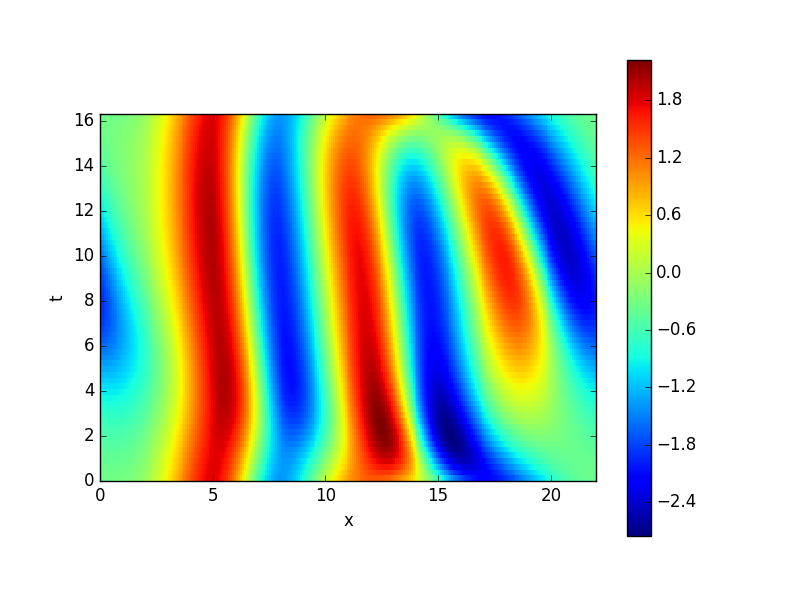
\includegraphics[width=\textwidth,height=.32\textheight]{MNGvndspacefinal2L}
\end{minipage}
\caption{ \label{fig:MNGspaceandtime1}
(a) Initial condition of the 16-by-16 space-by-time discretization of
\rpo{16.31}. $L_0 = 22$.
(b) Resulting periodic orbit after variational {newton descent} in time $L =
22, T = 15.7444884386$,
(c) resulting periodic orbit after variational {newton descent} in space.
%%%lost the number for final spatial size will need to run code again.
}
\end{figure}

As a means of cross-checking results I wrote variational {newton descent} code for time, debugged, and got it working. It follows the "direct-matrix" approach
that I have been finding useful.
The velocity equation takes the form
\beq \label{e-MNGkstimeDM}
v = Q_1 \cdot \utensor - Q_2 \cdot F \cdot ((F^{-1}\utensor) \star (F^{-1}\utensor))
\eeq
and the stability matrix is therefore
\beq
A = Q_1 - 2 * Q_2 * \cdot F \cdot diag(F^{-1}\utensor) \cdot F^{-1}
\eeq

\reffig{fig:MNGspaceandtime1} is a comparison between resulting orbits from both space and time variational {newton descent}.
The general structure of the resulting orbit is preserved even though the periods are quite different. At first I believed that
these were supporting evidence that something is going right but now I am confused. The spatial domain resulting from the \emph{spatial}
{newton descent} is largely unchanged, meaning that the orbit that results should be a unique solution with a unique period; but the \emph{time}
variational {newton descent} changes the period somewhat drastically, and because the spatial domain size is fixed this might mean that I am
finding the same solution but this is contradictory because the periods are so different. Also good evidence that there is something wrong is that
the \emph{time} {newton descent} is taking a \rpo\ initial condition and seemingly changing it into a periodic orbit? I don't know what
to think of it but I am glad that I rewrote the time {newton descent} code as it'll be a good stepping stone into whether or not I need to rewrite the equations
in a symmetry reduced form in order to find {\rpo}s or not. I think that's where I'm headed at least.

Began parsing through the literature on (variational) {newton descent},
specifically \refrefs{CvitLanCrete02,lanVar1} and for invariant tori
\refref{LCC06}.


\beq
\frac{\partial x}{\partial \tau}(s + \omega, \tau) + \frac{\partial x}{\partial s}
(s + \omega, \tau)\frac{\partial \omega}{\partial \tau}(\tau) - J(x(s,\tau))\frac{\partial x}{\partial \tau}(s,\tau) =
f(x (s,\tau))-x(s+\omega,\tau),
\ee{MNGNewtonDescent}


There is a storm in the distance however, as this general procedure is ruined for the spatial problem.
As we know from the chronotopic literature \refrefs{LePoTo96, LePoTo97, PoToLe98, GiLePo95},
that iteration in space typically does not converge to the same attractor as iteration in time,
and generally corresponds to a strange repeller. Therefore I cannot hope to form an initial guess
loop from using a Poincar\'e section in the spatial direction,
 as typically all of my Fourier coefficients go off to infinity before a recurrence is found.

My idea to remedy this is to actually use \emph{time} integration to form a initial guess loop for
applying {newton descent} in \emph{space}. If I integrate a spatially periodic initial condition in time,
by virtue of the spatial periodicity there is a close recurrence in the spatial direction
(close and not exact only due to discretization I believe). If I've thought about this the right way.
It's the smartest way I can think of to generate an initial condition for the spatial {newton descent}
\refeq{e-FksX} given that my spatial integration code is ill-behaved. If my \emph{spatial} code was
working and there is no lapse in my rationale then it might actually have been a way to produce smooth
initial guess loops for the \emph{time} direction {newton descent} code.

Past two days have been spent making changes to {newton descent} and testing
those changes. For any changes that I make that translate generically to
any system I try to test them with R\"ossler first before applying them
to antisymmetric subspace $\bbU^+$ of \KS. The other changes that are
unique to antisymmetric \KS\ must of course be tested in that realm. The
changes are looking promising, as I can find longer periodic orbits in
the R\"ossler system now, however the period seems to be slightly off
(Integrating the solution after application of {newton descent} yields a
solution that is periodic but overlaps). This is my number one suspect
for why the {newton descent} code continues to stall at the moment; however,
for the R\"ossler system although it is much slower for longer periodic
orbits, it still converges very quickly once $F^2 < 1$.

{\bf spatial {newton descent}} stalls out around
cost functional value $\mathcal{F}^2 \approx 10^{-8}$. Final configuration
space velocity field is a highly oscillating very non-physical
 type solution that looks like the result of aliasing; I believe I need
to incorporate more Fourier modes as a first step to fix the
 issue, or the number of discretization points, although doing so leads me
to run out of memory

I realized that I should not have to worry about implementing a slicing condition
in the spatial version of variational {newton descent}; All that was required in the
time case was to reduce the symmetry associated with the marginal direction parallel to
velocity, i.e. a Poincar\'e section. I didn't worry about the spatial translational invariance
and it was able to converge to a solution just fine in the time case.

In this line of thought, because space and time have their roles
reversed, I should only have to take into consideration the translational
invariance in the spatial direction and not the \SOn{2} symmetry in the (now periodic)
time direction.

I also changed the definition of the stability matrix elements that arise due
to the nonlinearity in hopes this will fix my problems; All in all, things are
working \emph{much} better than they were even when compared to yesterday,
although the convergence properties are still not where they need to be in
order to say I "found" an new solution yet (For an initial condition whose
initial cost functional value is $\mathcal{F}_0^2 \approx 5$ my code is able to
reduce it to $\mathcal{F}_{\tau}^2 \approx 10^{-1}$). I'm currently testing my
code with discretized versions of \ppo{10.2}, but I am going to try to see what
happens to an more general initial condition next.

There also might be a smarter way of choosing a constraint that enables better
convergence, as opposed to the ``first coordinate" hyperplane (i.e. the first
Fourier mode in most systems). I'm currently playing around with using a
hyperplane condition on the ``more dynamical" variables \MNGedit{which is a
hasty and crude name not to be taken seriously}. What I mean by this is that in
\refeq{e-FksX} the spatial derivatives of the Fourier coefficients of
$u^{(3)}$, which represents the third derivative, are much more complex than
the other derivatives, so perhaps using a hyperplane condition on one of these
coordinates would be better; this hasn't seemed to be the case yet.

Realized I made a small mistake when thinking about using Fourier transforms along
the parameterization direction in order to approximate the loop tangent space \refeq{e-FvndBAD}.
I thought that I would have to somehow permute the elements \refeq{e-FvndBAD} of the "Loop Vector" (vector that
encodes the parameterization of initial condition for periodic orbit search). The reasoning behind this
was in order to use differentiate with respect to a parameterization variable $s$, I would need
the elements to be in sequential order with respect in parameterization variable $s$, in order to
multiply by vector $i \vec{m}$, where $m$ is the conjugate variable (in a Fourier transform sense)
to $s$. This is \textbf{\emph{not}}
the case, as I can merely exploit the Kronecker outer product to produce a diagonal matrix such that
along the diagonal there are $M$ duplicates of each element of $\vec{m}$

We are essentially diagonalizing a sparse matrix for $\mathcal{O}(M\,(n log(n)))$ flops
from taking $M$ Fourier transforms of length $n =$~power~of~$2$.
This is all well and good, but I think that there might be complications from the stability matrices;
I need to go through the calculation, but the naive way to write the
stability matrices in their new representation is:
 $\tilde{\mathbf{A}} = \mathbf{F} \mathbf{A} \mathbf{F^{*}}$, where $F$
is a unitary matrix representing the discrete Fourier transform.

When you include the amount of flops needed to produce the product of these matrices, I don't think
the benefits outweigh the costs \emph{unless} a much smaller discretization can be used due to the
convergence of Fourier coefficients (i.e. a truncation in the parameterization variable).

Next is the representation of the fictitious time evolution as a system of linear equations, similar to
\refeq{e-MNGVNDpseudo}, which is restated here for comparison to the new system of equations.

The old linear system is given by,
\beq
\begin{bmatrix} M & -v \end{bmatrix}  \left[ \begin{array}{c} \delta \tilde{x} \\ \delta \lambda \end{array} \right] =
    \delta \tau \left[ \begin{array}{c} \lambda v - \tilde{v} \end{array} \right],
\eeq
where $M = D - \lambda Diag(A_n)$ with $D$ being the finite difference matrix, and $A_n$ a block diagonal matrix containing stability matrices.

Now, the equations the same form, with new variables described by over-bars
\beq \label{e-MNGVNDpseudoFMAT}
\begin{bmatrix} \bar{M} & -\bar{v} \end{bmatrix}  \left[ \begin{array}{c} \delta \tilde{\bar{x}} \\ \delta \bar{\lambda} \end{array} \right] =
    \delta \tau \left[ \begin{array}{c} \lambda \hat{\bar{v}} - \tilde{\bar{v}} \end{array} \right],
\eeq
where $\bar{M} = \mathbf{F} Diag (i \vec{m}) \mathbf{F}^* \otimes \mathbf{I}_d - \lambda Diag(A_n)$
%$\bar{M} = Diag (i \vec{m}) \otimes \mathbf{I}_d - \lambda \mathbf{F} Diag(A_n) \mathbf{F}^*$,
and $\bar{v} = \mathcal{F}(v)$, $\tilde{\bar{v}} = (Diag(i \vec{m})* \tilde{\bar{x}}$.
\MNG{}{I changed this such that the only difference
between my current code and this formulation
 is the calculation of approximate tangent space via Fourier methods.}

{\bf Spatial {\Descent}}
Rewrote the main body of the fictitious time evolution loop to hopefully deal
with memory management a bit better, but still getting memory issues.
Waiting on latest Arnoldi iteration to finish before using terminal to do calculations.

Waffling between implementation of least squares solver for pseudoinverse variational
{newton descent}.

GMRES seems to be locked by memory.
Also tried to implement QR decomposition as in Trefethen\r{Trefethen97}
but trying to stick to pseudoinverse and least squares solvers as they
typically work better; also keeping track of large matrices is a downside.

The best results, (i.e. better than square matrix problem, but still not
good enough) was with SciPy's LSQR algorithm, which, in the paper that
it is based on \refref{PaSaLSQR}, describes it as a ``conjugate-gradient-like" algorithm,
with better stability. I haven't gotten into the nitty gritty as of yet.

A useful class of numerical methods often used in optimization\rf{BoyVan04, Dennis96} are known
as \textit{descent methods}. In our context, optimization denotes the numerical process
of finding minimizers of a scalar valued cost function which vector valued inputs, the \spt\
Fourier modes and \spt\ parameters. Broadly speaking, descent methods are numerical methods
which iteratively solve unconstrained optimization. These methods accomplish this by one
way or another providing a direction to step in which monotonically decreases the value of
the cost functional, hence ``descent'' (assuming a non-negative scalar cost function).
The method with which to compute the descent direction is the distinguishing property
between descent methods. In the limit of an infinitesimal step size, the iterative descent
can be characterized as a fictitious flow with respect to a fictitious time\rf{LCC06}.
The advantages of descent methods are that they do not require the construction nor
the inversion of any matrices. The computational and memory requirements
are relatively cheap in comparison to direct methods but the trade off is the
rate of convergence. The convergence of a descent method
is guaranteed but only in the impractical limit of infinite fictitious time.
There are some tools for improving the rate of convergence such as preconditioning
operators which will be discussed in a later section.


\beq
\frac{\partial x}{\partial \tau}(s + \omega, \tau) + \frac{\partial x}{\partial s}
(s + \omega, \tau)\frac{\partial \omega}{\partial \tau}(\tau) - J(x(s,\tau))\frac{\partial x}{\partial \tau}(s,\tau) =
f(x (s,\tau))-x(s+\omega,\tau),
\ee{MNGNewtonDescent}


The old linear system is given by,
\beq
\begin{bmatrix} M & -v \end{bmatrix}  \left[ \begin{array}{c} \delta \tilde{x} \\ \delta \lambda \end{array} \right] =
    \delta \tau \left[ \begin{array}{c} \lambda v - \tilde{v} \end{array} \right],
\eeq
where $M = D - \lambda Diag(A_n)$ with $D$ being the finite difference matrix, and $A_n$ a block diagonal matrix containing stability matrices.

Now, the equations the same form, with new variables described by over-bars
\beq \label{e-MNGVNDpseudoFMAT}
\begin{bmatrix} \bar{M} & -\bar{v} \end{bmatrix}  \left[ \begin{array}{c} \delta \tilde{\bar{x}} \\ \delta \bar{\lambda} \end{array} \right] =
    \delta \tau \left[ \begin{array}{c} \lambda \hat{\bar{v}} - \tilde{\bar{v}} \end{array} \right],
\eeq

where $\bar{M} = \mathbf{F} Diag (i \vec{m}) \mathbf{F}^* \otimes \mathbf{I}_d - \lambda Diag(A_n)$
%$\bar{M} = Diag (i \vec{m}) \otimes \mathbf{I}_d - \lambda \mathbf{F} Diag(A_n) \mathbf{F}^*$,
and $\bar{v} = \mathcal{F}(v)$, $\tilde{\bar{v}} = (Diag(i \vec{m})* \tilde{\bar{x}}$.
\MNG{}{I changed this such that the only difference
between my current code and this formulation
 is the calculation of approximate tangent space via Fourier methods.}
e are essentially diagonalizing a sparse matrix for $\mathcal{O}(M\,(n log(n)))$ flops
from taking $M$ Fourier transforms of length $n =$~power~of~$2$.
This is all well and good, but I think that there might be complications from the stability matrices;
I need to go through the calculation, but the naive way to write the
stability matrices in their new representation is:
 $\tilde{\mathbf{A}} = \mathbf{F} \mathbf{A} \mathbf{F^{*}}$, where $F$
is a unitary matrix representing the discrete Fourier transform.

When you include the amount of flops needed to produce the product of these matrices, I don't think
the benefits outweigh the costs \emph{unless} a much smaller discretization can be used due to the
convergence of Fourier coefficients (i.e. a truncation in the parameterization variable).

Next is the representation of the fictitious time evolution as a system of linear equations, similar to
\refeq{e-MNGVNDpseudo}, which is restated here for comparison to the new system of equations.

\begin{figure}[ht]
\begin{minipage}[height=.32\textheight]{.45\textwidth}
\centering \small{\texttt{(a)}}
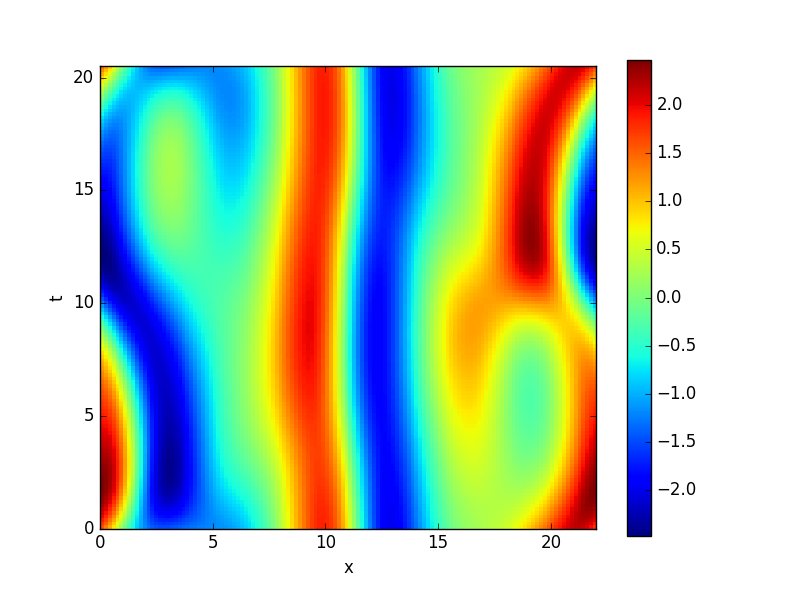
\includegraphics[width=\textwidth,height=.32\textheight]{MNGspacetimeinit1}
\end{minipage}
\begin{minipage}[height=.32\textheight]{.45\textwidth}
\centering \small{\texttt{(b)}}
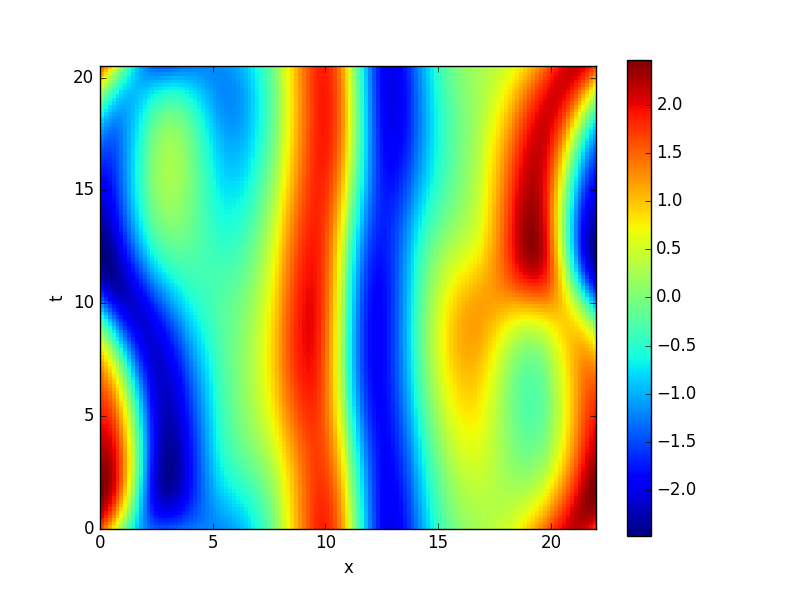
\includegraphics[width=\textwidth,height=.32\textheight]{MNGspacetimefinal1}
\end{minipage}
\caption{ \label{fig:MNGspacetime11}
(a) Initial condition of the 32-by-32 space-by-time discretization of \ppo{10.2}:
$(L_0,\period{0}) = (L_0, 2\period{p_0})= (22,20.5057459345)$.
(b) Resulting spatiotemporal fixed point
$(L_p,2\period{p}) =  (22.0000104401, 20.5057499188)$
}
\end{figure}


The best results, (i.e. better than square matrix problem, but still not
good enough) was with SciPy's LSQR algorithm, which, in the paper that
it is based on \refref{PaSaLSQR}, describes it as a ``conjugate-gradient-like" algorithm,
with better stability. I haven't gotten into the nitty gritty as of yet.

While waiting for Arnoldi iteration to finish so that I could begin testing the
spatial variational {newton descent} without fear of memory problems I was trying to
think about the best way to use \refeq{e-FksSpattemp}, which I will restate
here.

First, $\utensor_{k,\ell}$ represents matrix elements, so it makes sense
to rewrite the equation as a matrix equation. Define matrices
$\mathbf{Q}_1 \equiv Diag(-q_k^2 +q_k^4)$,
$\mathbf{W} \equiv Diag(i \omega_\ell)$,
$\mathbf{Q}_2 \equiv Diag(\frac{i q_k}{2})$, and let
the two dimensional FFT be represented by matrix multiplication
$\mathbf{U} = \mathbf{F}_M \mathbf{u} \mathbf{F}_N$,
where the matrix elements $U_{k,\ell} = \utensor_{k,\ell}$.

and therefore we have an equation of the form:
$f_{k,\ell}(\utensor_{k,\ell})-\utensor_{k,\ell} = 0$,
where the \jacobianM\ is given by the fourth rank tensor that arises from taking partial derivatives with
respect to $\utensor_{k,\ell}$
More to be derived in the future, hoping to make headway into finding tori; I can't tell if this equation
is going to be useful or if I should really be working towards deriving and learning variational {newton descent}
equations for finding tori similar to Lan, Chandre and Cvitanovi{\'c}\rf{LCC06}.

Application of the spatial {newton descent} code to ergodic trajectories that have been deformed to
be periodic in time were resulting in the "falling into equilibrium" problem, this was due to a bug
where the wrong temporal system sizes were being used.

Application of spatial {newton descent} on \ppo{10.2} results in a reduced cost
functional but seems rather obstinate in regards to convergence. Luckily, the
approximate loop seems to fluctuate around spatial extent $L=22$. I think this
is a good indication as it means the spatial {newton descent} is capturing the
spatial geometry of \ppo{10.2}. That is to say, even while reducing the cost
functional the solution doesn't want to betray itself, as it originates from
the spatial system size $L=22$.

I tried whether it be the error tolerances, step sizes (variable or constant), initial condition
discretizations, least squares solvers, pseudoinverse or regular inverse methods, hypersurface constraints,
matrix preconditioners, etc, did not help the converge properties.
By examining the corrections being applied to deform the loop, specifically the maximum correction applied
in each step it seems most of the steps are modifying the "period" i.e. the spatial extent of the initial
condition the most. There might be some way to discourage this with an additional condition on the
rescaling factor $\lambda$ that matches the magnitudes of the approximate tangent space to the
actual tangent space.


I believe I got it working finally, however, the results so far aren't as
interesting as I had dreamed. I finished this at the end of the day so I didn't
get to test it too much, but so far there are two resulting possibilities.
First, with a time periodic initial condition, i.e. one of the periodic orbits
in time of \KS, when allowing for spatial domain changes and changes to the
temporal Fourier coefficients, the solution (only tested one so far) converged
to one of the temporal equilibria of the \KS\ system. This I believe is an
indication that my code is indeed working, even though this was usually a sign
of numerical issues when searching for periodic orbits in time using the
variational methods, (i.e. the only way to reduce the cost functional
$\mathcal{F}^2 = \lambda v - \tilde{v}$ is to send $v$ and $\tilde{v}$ to $0$.
The reason I believe this is still valid is because the spatial derivatives of
the equilibrium state found are nonzero; i.e. one of the "spatial periodic
orbits" I have found is indeed the temporal equilibrium of the system.


After more investigation it turns out that the spatial variational code is indeed not working yet. Tried to put
resulting orbits into time integrator in order to reproduce the result and got an unmatching solution.
\reffig{fig:MNGvndspace2} is my
newest "results". It uses a \RPO{16.31} of the \KSe\ as the initial condition. I think I was deceived by how nice it looks
I suppose...couldn't find any errors today that could enable reproduction via time integration.

As an additional test I put the solutions into Burak's symmetry reduced time integrator to verify whether
the "solution" in \reffig{fig:MNGvndspace2} was a \rpo\ but alas there was no luck; there is some other error
that I haven't been able to identify as of yet.
Found another negative sign error, updating \reffig{fig:MNGvndspace1}.


\begin{figure}
\begin{minipage}[height=.32\textheight]{.45\textwidth}
\centering \small{\texttt{(a)}}
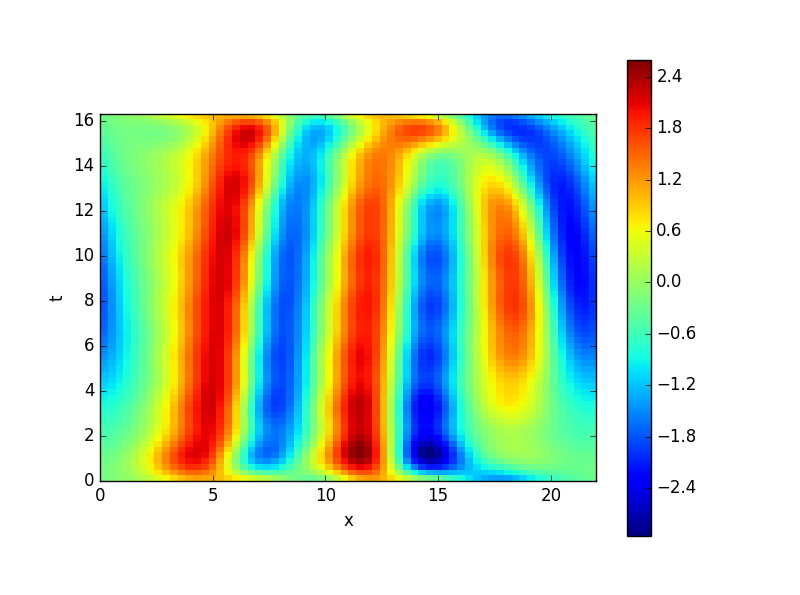
\includegraphics[width=\textwidth,height=.32\textheight]{MNGvndspaceinit2}
\end{minipage}
\\
\begin{minipage}[height=.32\textheight]{.45\textwidth}
\centering \small{\texttt{(b)}}
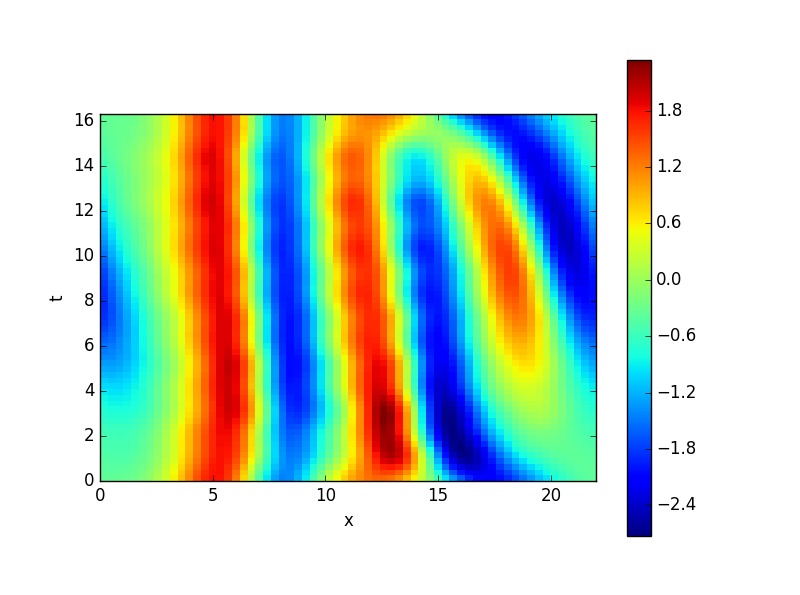
\includegraphics[width=\textwidth,height=.32\textheight]{MNGvndtimefinal2}
\end{minipage}
\begin{minipage}[height=.32\textheight]{.45\textwidth}
\centering \small{\texttt{(c)}}
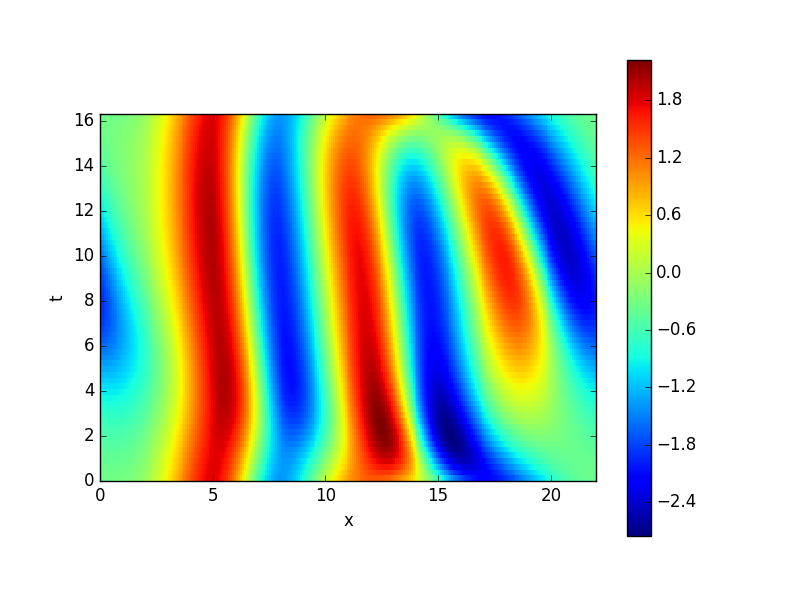
\includegraphics[width=\textwidth,height=.32\textheight]{MNGvndspacefinal2L}
\end{minipage}
\caption{ \label{fig:MNGspaceandtime1}
(a) Initial condition of the 16-by-16 space-by-time discretization of
\rpo{16.31}. $L_0 = 22$.
(b) Resulting periodic orbit after variational {newton descent} in time $L =
22, T = 15.7444884386$,
(c) resulting periodic orbit after variational {newton descent} in space.
%%%lost the number for final spatial size will need to run code again.
}
\end{figure}

As a means of cross-checking results I wrote variational {newton descent} code for time, debugged, and got it working. It follows the "direct-matrix" approach
that I have been finding useful.
The velocity equation takes the form

\reffig{fig:MNGspaceandtime1} is a comparison between resulting orbits from both space and time variational {newton descent}.
The general structure of the resulting orbit is preserved even though the periods are quite different. At first I believed that
these were supporting evidence that something is going right but now I am confused. The spatial domain resulting from the \emph{spatial}
{newton descent} is largely unchanged, meaning that the orbit that results should be a unique solution with a unique period; but the \emph{time}
variational {newton descent} changes the period somewhat drastically, and because the spatial domain size is fixed this might mean that I am
finding the same solution but this is contradictory because the periods are so different. Also good evidence that there is something wrong is that
the \emph{time} {newton descent} is taking a \rpo\ initial condition and seemingly changing it into a periodic orbit? I don't know what
to think of it but I am glad that I rewrote the time {newton descent} code as it'll be a good stepping stone into whether or not I need to rewrite the equations
in a symmetry reduced form in order to find {\rpo}s or not. I think that's where I'm headed at least.


\begin{figure}[ht]
\begin{minipage}[height=.32\textheight]{.45\textwidth}
\centering \small{\texttt{(a)}}
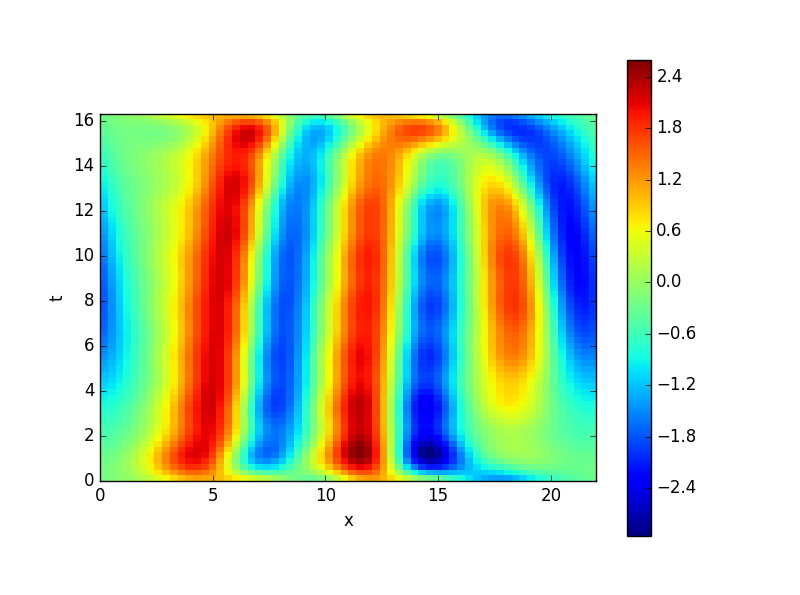
\includegraphics[width=\textwidth,height=.32\textheight]{MNGvndspaceinit2}
\end{minipage}
\begin{minipage}[height=.32\textheight]{.45\textwidth}
\centering \small{\texttt{(b)}}
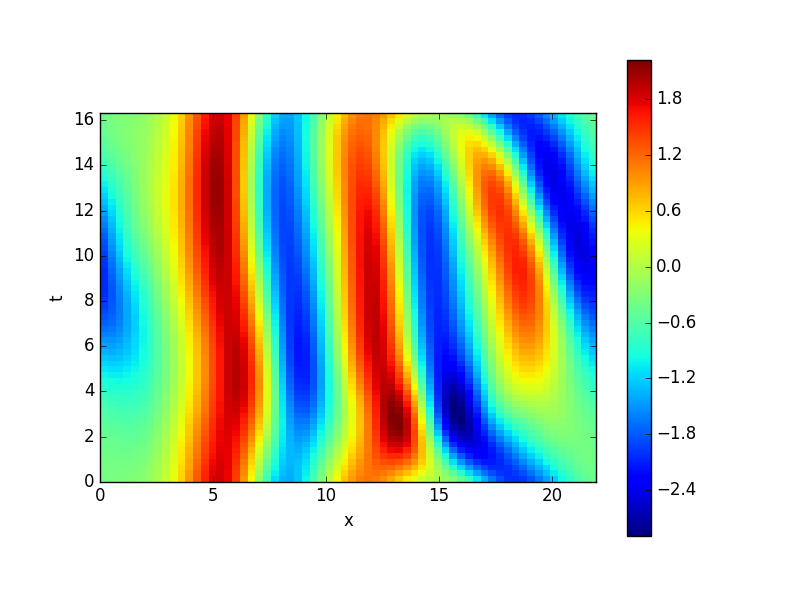
\includegraphics[width=\textwidth,height=.32\textheight]{MNGvndspacefinal2}
\end{minipage}
\caption{ \label{fig:MNGvndspace2}
(a) Initial condition of the 16-by-16 space-by-time discretization of \RPO{16.31} ($L=22$) for spatial
variational {newton descent} of the \KSe\ (b)Resulting "spatial periodic orbit" (temporal equilibrium), with
final spatial extent of $L = 21.9394614064$
}
\end{figure}
\begin{figure}[ht]
\begin{minipage}[height=.32\textheight]{.45\textwidth}
\centering \small{\texttt{(a)}}
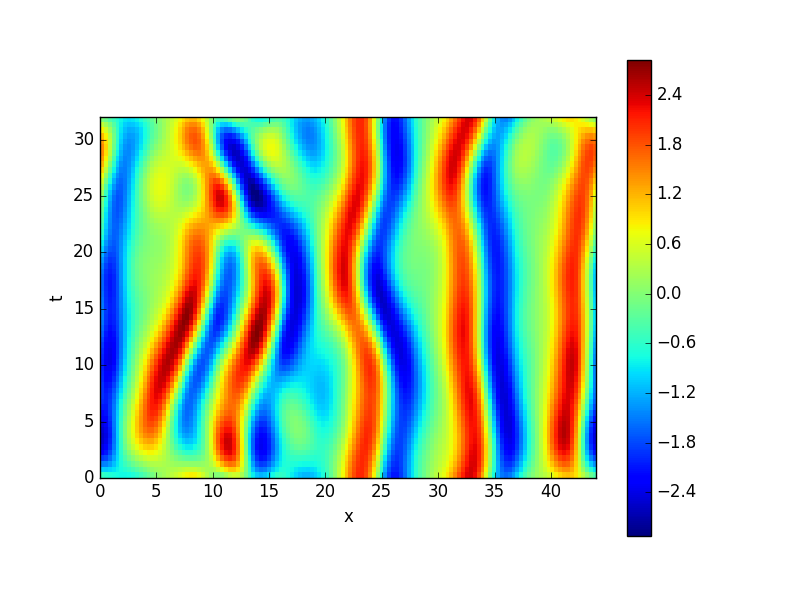
\includegraphics[width=\textwidth,height=.32\textheight]{MNGvndspaceinit3}
\end{minipage}
\begin{minipage}[height=.32\textheight]{.45\textwidth}
\centering \small{\texttt{(b)}}
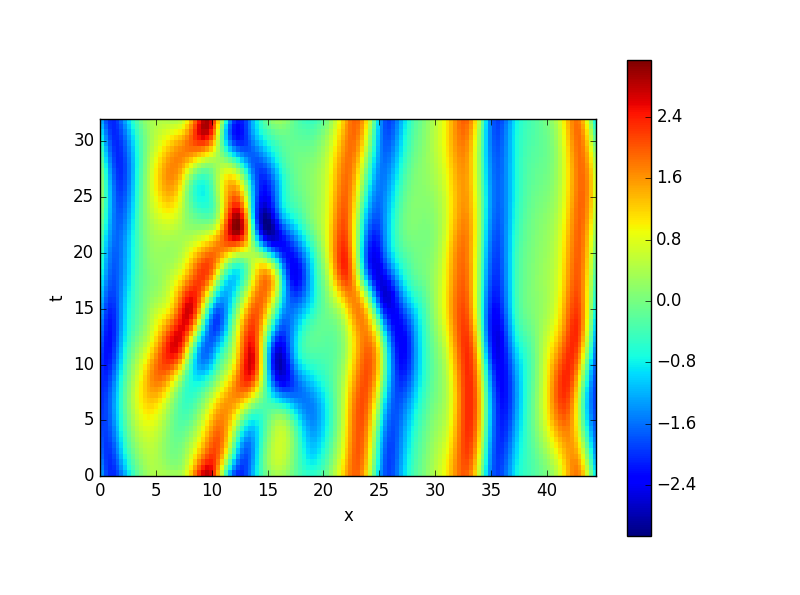
\includegraphics[width=\textwidth,height=.32\textheight]{MNGvndspacefinal3}
\end{minipage}
\caption{ \label{fig:MNGvndspace3}
(a) Initial condition of the 32-by-16 space-by-time discretization of a piece
of an ergodic trajectory that has been deformed to be periodic in time. $L=44$.
(b) Resulting spatiotemporal \po, with
final spatial extent of $L = 44.3937151766$.
}
\end{figure}


updated \reffig{fig:MNGvndspace2}, \reffig{fig:MNGvndspace1}, and uploaded \reffig{fig:MNGvndspace3} to display
current results.

After trying numerous small modifications to the variational method's system
of equations from \refref{LanThesis} including implementing factors involving
the coordinate involved in defining the in-slice time and other quantities
involving the slice tangents I didn't get any improvements over what I already
had. I still think the problem has to do with the slice time so I went over
the derivation of the equations and I believe I found a correction that can be
made.

\beq \nonumber
D_{\mathcal{F}} = \mathbf{P}^{-1}\mathbf{F}^{-1}\mathbf{Diag}(is)\mathbf{F}\mathbf{P} \quad
    \mbox{where,}
\label{e-FvndBAD}
\eeq

$\mathbf{F}$ = Block diagonal matrix composed of Fourier transform matrices (i.e. to Fourier transform each
of the Fourier coefficient series with respect to parameterization variable), $\mathbf{P}$ = Permutation matrix
to reorder in specific way to enable easy Fourier transforms.

Another main challenge is how to implement a slice condition to deal with translational
invariance. Typically this is dealt with when the spatial Fourier series is being used, and
therefore it is easier to represent a hypersurface that eliminates this marginal direction; in
the spatial {newton descent} code (this is what I call using \refeq{e-FksX} with variational
{newton descent}) I am trying to eliminate the translational freedom but it's not as straightforward as
the {\fFslice}; as the {\fFslice} in this case would eliminate time translations.
I've been looking towards some of the papers about invariant tori and their "phase conditions" as a
possible means of escape.

I realized that I should not have to worry about implementing a slicing condition
in the spatial version of variational {newton descent}; All that was required in the
time case was to reduce the symmetry associated with the marginal direction parallel to
velocity, i.e. a Poincar\'e section. I didn't worry about the spatial translational invariance
and it was able to converge to a solution just fine in the time case.

I thought that I would have to somehow permute the elements \refeq{e-FvndBAD} of the "Loop Vector" (vector that
encodes the parameterization of initial condition for periodic orbit search). The reasoning behind this
was in order to use differentiate with respect to a parameterization variable $s$, I would need
the elements to be in sequential order with respect in parameterization variable $s$, in order to
multiply by vector $i \vec{m}$, where $m$ is the conjugate variable (in a Fourier transform sense)
to $s$. This is \textbf{\emph{not}}
the case, as I can merely exploit the Kronecker outer product to produce a diagonal matrix such that
along the diagonal there are $M$ duplicates of each element of $\vec{m}$

We are essentially diagonalizing a sparse matrix for $\mathcal{O}(M\,(n log(n)))$ flops
from taking $M$ Fourier transforms of length $n =$~power~of~$2$.
This is all well and good, but I think that there might be complications from the stability matrices;
I need to go through the calculation, but the naive way to write the
stability matrices in their new representation is:
 $\tilde{\mathbf{A}} = \mathbf{F} \mathbf{A} \mathbf{F^{*}}$, where $F$
is a unitary matrix representing the discrete Fourier transform.

Next is the representation of the fictitious time evolution as a system of linear equations, similar to
\refeq{e-MNGVNDpseudo}, which is restated here for comparison to the new system of equations.

The old linear system is given by,
\beq
\begin{bmatrix} M & -v \end{bmatrix}  \left[ \begin{array}{c} \delta \tilde{x} \\ \delta \lambda \end{array} \right] =
    \delta \tau \left[ \begin{array}{c} \lambda v - \tilde{v} \end{array} \right],
\eeq
where $M = D - \lambda Diag(A_n)$ with $D$ being the finite difference matrix, and $A_n$ a block diagonal matrix containing stability matrices.

Now, the equations the same form, with new variables described by over-bars
\beq \label{e-MNGVNDpseudoFMAT}
\begin{bmatrix} \bar{M} & -\bar{v} \end{bmatrix}  \left[ \begin{array}{c} \delta \tilde{\bar{x}} \\ \delta \bar{\lambda} \end{array} \right] =
    \delta \tau \left[ \begin{array}{c} \lambda \hat{\bar{v}} - \tilde{\bar{v}} \end{array} \right],
\eeq
where $\bar{M} = \mathbf{F} Diag (i \vec{m}) \mathbf{F}^* \otimes \mathbf{I}_d - \lambda Diag(A_n)$
%$\bar{M} = Diag (i \vec{m}) \otimes \mathbf{I}_d - \lambda \mathbf{F} Diag(A_n) \mathbf{F}^*$,
and $\bar{v} = \mathcal{F}(v)$, $\tilde{\bar{v}} = (Diag(i \vec{m})* \tilde{\bar{x}}$.
\MNG{}{I changed this such that the only difference
between my current code and this formulation
 is the calculation of approximate tangent space via Fourier methods.}


Next is the representation of the fictitious time evolution as a system of linear equations, similar to
\refeq{e-MNGVNDpseudo}, which is restated here for comparison to the new system of equations.

The old linear system is given by,
\beq
\begin{bmatrix} M & -v \end{bmatrix}  \left[ \begin{array}{c} \delta \tilde{x} \\ \delta \lambda \end{array} \right] =
    \delta \tau \left[ \begin{array}{c} \lambda v - \tilde{v} \end{array} \right],
\eeq
where $M = D - \lambda Diag(A_n)$ with $D$ being the finite difference matrix, and $A_n$ a block diagonal matrix containing stability matrices.

Now, the equations the same form, with new variables described by over-bars
\beq \label{e-MNGVNDpseudoFMAT}
\begin{bmatrix} \bar{M} & -\bar{v} \end{bmatrix}  \left[ \begin{array}{c} \delta \tilde{\bar{x}} \\ \delta \bar{\lambda} \end{array} \right] =
    \delta \tau \left[ \begin{array}{c} \lambda \hat{\bar{v}} - \tilde{\bar{v}} \end{array} \right],
\eeq
where $\bar{M} = \mathbf{F} Diag (i \vec{m}) \mathbf{F}^* \otimes \mathbf{I}_d - \lambda Diag(A_n)$
%$\bar{M} = Diag (i \vec{m}) \otimes \mathbf{I}_d - \lambda \mathbf{F} Diag(A_n) \mathbf{F}^*$,
and $\bar{v} = \mathcal{F}(v)$, $\tilde{\bar{v}} = (Diag(i \vec{m})* \tilde{\bar{x}}$.
\MNG{}{I changed this such that the only difference
between my current code and this formulation
 is the calculation of approximate tangent space via Fourier methods.}

